\documentclass{report}

\input{~/dev/latex/template/preamble.tex}
\input{~/dev/latex/template/macros.tex}

\title{\Huge{}}
\author{\huge{Nathan Warner}}
\date{\huge{}}
\pagestyle{fancy}
\fancyhf{}
\lhead{Warner \thepage}
\rhead{}
% \lhead{\leftmark}
\cfoot{\thepage}
%\setborder
% \usepackage[default]{sourcecodepro}
% \usepackage[T1]{fontenc}

\begin{document}
    % \maketitle
        \begin{titlepage}
       \begin{center}
           \vspace*{1cm}
    
           \textbf{Calculus 2} \\
           Chapter 6
    
           \vspace{0.5cm}
            
                
           \vspace{1.5cm}
    
           \textbf{Nathan Warner}
    
           \vfill
                
                
           \vspace{0.8cm}
         
           
\includegraphics[width=0.4\textwidth]{~/niu/seal.png}
                
           Computer Science \\
           Northern Illinois University\\
           October 27, 2023 \\
           United States\\
           
                
       \end{center}
    \end{titlepage}
    \tableofcontents
    \pagebreak \bigbreak \noindent
    \vspace{2in} \\
    \begin{Huge}
       \textbf{Power Series} 
    \end{Huge}
    \bigbreak \noindent 
    \line(1,0){490}
    \bigbreak \noindent 
    \phantomsection
    \addcontentsline{toc}{section}{6.1 Power Series and Functions}
    \section*{6.1 Power Series and Functions}
    \bigbreak \noindent 
    A power series is a type of series with terms involving a variable. More specifically, if the variable is x, then all the terms of the series involve powers of x. As a result, a power series can be thought of as an infinite polynomial. Power series are used to represent common functions and also to define new functions. In this section we define power series and show how to determine when a power series converges and when it diverges. We also show how to represent certain functions using power series.
    \bigbreak \noindent 
    \phantomsection
    \addcontentsline{toc}{subsection}{Form of a Power Series}
    \subsection*{Form of a Power Series}
    \bigbreak \noindent 
    \begin{dfn}[Power series]
        A series of the form
    \begin{align*}
        \sum_{n=0}^{\infty} c_n x^n &= c_0 + c_1 x + c_2 x^2 + \cdots 
    .\end{align*}
    is a power series centered at \( x = 0 \).
    \bigbreak \noindent 
    A series of the form
    \begin{align*}
        \sum_{n=0}^{\infty} c_n (x - a)^n &= c_0 + c_1 (x - a) + c_2 (x - a)^2 + \cdots 
    .\end{align*}
    is a power series centered at \( x = a \).
    \end{dfn}
    
    \bigbreak \noindent 
    To make this definition precise, we stipulate that \( x^0 = 1 \) and \( (x - a)^0 = 1 \) even when \( x = 0 \) and \( x = a \), respectively.
    \bigbreak \noindent 
    The series
    \begin{align*}
        \sum_{n=0}^{\infty} \frac{x^n}{n!} &= 1 + x + \frac{x^2}{2!} + \frac{x^3}{3!} + \cdots
    \end{align*}
    and
    \begin{align*}
        \sum_{n=0}^{\infty} n! x^n &= 1 + x + 2! x^2 + 3! x^3 + \cdots
    \end{align*}
    are both power series centered at \( x = 0 \).
    \bigbreak \noindent 
    The series
    \begin{align*}
        \sum_{n=0}^{\infty} \frac{(x - 2)^n}{(n + 1)3^n} &= 1 + \frac{x - 2}{2 \cdot 3} + \frac{(x - 2)^2}{3 \cdot 3^2} + \frac{(x - 2)^3}{4 \cdot 3^3} + \cdots
    \end{align*}
    is a power series centered at \( x = 2 \).

    \bigbreak \noindent 
    \phantomsection
    \addcontentsline{toc}{subsection}{Convergence of a Power Series}
    \subsection*{Convergence of a Power Series}
    \bigbreak \noindent 
    \begin{thrmm}[Convergence of a Power Series]
        Consider the power series \(\sum_{n=0}^{\infty} c_n (x - a)^n\). The series satisfies exactly one of the following properties:
        \begin{enumerate}[label=(\roman*)]
            \item The series converges at \( x = a \) and diverges for all \( x \neq a \).
            \item The series converges for all real numbers \( x \).
            \item There exists a real number \( R > 0 \) such that the series converges if \( |x - a| < R \) and diverges if \( |x - a| > R \). At the values \( x \) where \( |x - a| = R \), the series may converge or diverge.
        \end{enumerate}
    \end{thrmm}
    \bigbreak \noindent 
    \begin{dfn}
        Consider the power series \(\sum_{n=0}^{\infty} c_n (x - a)^n\). The set of real numbers \( x \) where the series converges is the interval of convergence. If there exists a real number \( R > 0 \) such that the series converges for \( |x - a| < R \) and diverges for \( |x - a| > R \), then \( R \) is the radius of convergence. If the series converges only at \( x = a \), we say the radius of convergence is \( R = 0 \). If the series converges for all real numbers \( x \), we say the radius of convergence is \( R = \infty \) (Figure 6.2).
    \end{dfn}
    \bigbreak \noindent 
    \begin{center}
        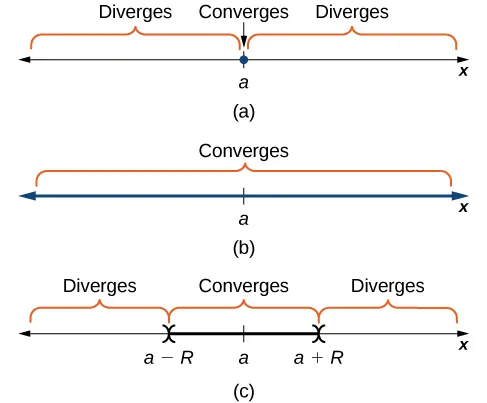
\includegraphics[scale=0.5]{./figures/popp.png}
    \end{center}

    \pagebreak \bigbreak \noindent 
    \begin{exm}
        Find the interval and radius of convergence
        \begin{align*}
            \summation{\infty}{n=1}\ \frac{x^{n}}{n!}\ 
        .\end{align*}
    \end{exm}
    \bigbreak \noindent 
    \textit{Solution.} For this, we use the ratio test and get
    \begin{align*}
        &\rho = \lim\limits_{n \to \infty}{\bigg\lvert \frac{\frac{x^{n}\cdot x}{n!(n+1)}}{\frac{n!}{x^{n}}} \bigg\rvert} \\
        &=\abs{x}\lim\limits_{n \to \infty}{\frac{1}{n+1}} \\
        &=0
    .\end{align*}
    \bigbreak \noindent 
    Since $ 0 \leq \rho  < 1$, this series will converge $\forall\ x \in \mathbb{R} $. Thus, the interval of convergence is $(-\infty,+\infty) $ and the radius of convergence is $R = \infty $

    \bigbreak \noindent 
    \begin{exm}
         Find the interval and radius of convergence
         \begin{align*}
             \summation{\infty}{n=0}\ n!x^{n}\ 
         .\end{align*}
    \end{exm}
    \bigbreak \noindent 
    \textit{Solution.} Again, we use the ratio test
    \begin{align*}
        &\rho = \lim\limits_{n \to \infty}{\frac{n!(n+1)x^{n}x}{n!x^{n}}} \\
        &=\abs{x}\lim\limits_{n \to \infty}{(n+1)} \\
        &=\infty
    .\end{align*}
    \bigbreak \noindent 
    Since $\rho = \infty $ The series diverges for all \( x \neq 0 \). Since the series is centered at \( x = 0 \), it must converge there, so the series converges only for \( x = 0 \). The interval of convergence is the single value \( x = 0 \) and the radius of convergence is \( R = 0 \).

    \pagebreak \bigbreak \noindent 
    \begin{exm}
        Find the interval and radius of convergence
        \begin{align*}
            \summation{\infty}{n=0}\ \frac{(x-2)^{n}}{(n+1)3^{n}}\ 
        .\end{align*}
    \end{exm}
    \bigbreak \noindent 
    \textit{Solution.} After applying the ratio test, we get
    \begin{align*}
        &\rho = \abs{x-2}\lim\limits_{n \to \infty}{\frac{n+1}{3n+2}} \\
        &=\frac{\abs{x-2}}{3}
    .\end{align*}
    \bigbreak \noindent 
    The question we ask is... when is this quantity $<1 $. 
    \begin{align*}
        &\frac{\abs{x-2}}{3} < 1 \\
        &\abs{x-2} < 3 \\
        &\implies -3 < x-2 < 3 \\
        &-1 < x < 5
    .\end{align*}
    \bigbreak \noindent 
    Thus, when $-1 < x < 5$, the series will converge absolutely. Likewise
    \begin{align*}
        &\frac{\abs{x-2}}{3} > 1 \\
        &\abs{x-2} > 3 \\
        \implies &x-2 < -3 \quad \text{ or } x-2 > 3 \\
        &x < -1 \quad \text{ or } x > 5
    .\end{align*}
    \bigbreak \noindent 
    Thus, the series will diverge if $x < -1$ or $x > 5$. Finally, we examine if $\rho = 1$
    \begin{align*}
        \frac{\abs{x-2}}{3} &= 1 \\
        \abs{x-2} &= 3 \\
        x-2 = 3 \quad &\quad x-2 = -3 \\
        x=5 \quad &\quad x=-1
    .\end{align*}
    \bigbreak \noindent 
    Thus, the ratio test is inconclusive for $x = -1$ or $x=5$. We need to test these values of $x$ separately. For $x=-1$ the series is given by
    \begin{align*}
        &\summation{\infty}{n=0}\ \frac{(-3)^{n}}{(n+1)3^{n}}\  \\
        &=\summation{\infty}{n=0}\ \frac{3^{n}(-1)^{n}}{(n+1)3^{n}}\  \\
        &=\summation{\infty}{n=0}\ \frac{(-1)^{n}}{n+1}\  
    .\end{align*}
    \bigbreak \noindent 
    Since this is the alternating harmonic series, it converges. Thus, the series converges at  $x=-1$. For $x=5$, the series is given by
    \begin{align*}
        &\summation{\infty}{n=0}\ \frac{3^{n}}{(n+1)3^{n}}\  \\
        &\summation{\infty}{n=0}\ \frac{1}{n+1}\ 
    .\end{align*}
    This is the harmonic series, which is divergent. Therefore, the power series diverges at \( x = 5 \). We conclude that the interval of convergence is \([ -1, 5 )\) and the radius of convergence is \( R = 3 \).

    \bigbreak \noindent 
    \phantomsection
    \addcontentsline{toc}{subsection}{Representing Functions as Power Series}
    \subsection*{Representing Functions as Power Series}
    \bigbreak \noindent 
    Being able to represent a function by an “infinite polynomial” is a powerful tool. Polynomial functions are the easiest functions to analyze, since they only involve the basic arithmetic operations of addition, subtraction, multiplication, and division. If we can represent a complicated function by an infinite polynomial, we can use the polynomial representation to differentiate or integrate it. In addition, we can use a truncated version of the polynomial expression to approximate values of the function. So, the question is, when can we represent a function by a power series?
    \bigbreak \noindent 
    Consider again the geometric series
\begin{equation}
    1 + x + x^2 + x^3 + \cdots = \sum_{n=0}^{\infty} x^n 
\end{equation}
Recall that the geometric series
\[
    a + ar + ar^2 + ar^3 + \cdots
\]
converges if and only if \( |r| < 1 \). In that case, it converges to \(\frac{a}{1 - r}\). Therefore, if \( |x| < 1 \), the series in Example 6.3 converges to \(\frac{1}{1 - x}\) and we write
\[
    1 + x + x^2 + x^3 + \cdots = \frac{1}{1 - x} \quad \text{for} \quad |x| < 1.
\]
As a result, we are able to represent the function \( f(x) = \frac{1}{1 - x} \) by the power series
\[
    1 + x + x^2 + x^3 + \cdots \quad \text{when} \quad |x| < 1.
\]
We now show graphically how this series provides a representation for the function \( f(x) = \frac{1}{1 - x} \) by comparing the graph of \( f \) with the graphs of several of the partial sums of this infinite series.

    \bigbreak \noindent 
    \begin{exm}
       Use a power series to represent each of the following functions  $f$. Find the interval of convergence. 
       \begin{align*}
           f(x) = \frac{1}{1+x^{3}}
       .\end{align*}
    \end{exm}
    \bigbreak \noindent 
    \textit{Solution.} should recognize this function $f$ as the sum of a geometric series, because
    \begin{align*}
        \frac{1}{1+x^{3}} = \frac{1}{1-(-x^{3})}
    .\end{align*}
    Using the fact that, for \( |r| < 1 \), \(\frac{a}{1 - r}\) is the sum of the geometric series
\[
    \sum_{n=0}^{\infty} ar^n = a + ar + ar^2 + \cdots,
\]
we see that, for \( \left| -x^3 \right| < 1 \),
\[
    \frac{1}{1 + x^3} = \frac{1}{1 - (-x^3)} = \sum_{n=0}^{\infty} (-x^3)^n = 1 - x^3 + x^6 - x^9 + \cdots.
\]
Since this series converges if and only if \( \left| -x^3 \right| < 1 \), the interval of convergence is \( (-1, 1) \), and we have
\[
    \frac{1}{1 + x^3} = 1 - x^3 + x^6 - x^9 + \cdots \quad \text{for} \quad |x| < 1.
\]


    \pagebreak \bigbreak \noindent 
    \begin{exm}
       Use a power series to represent each of the following functions  $f$. Find the interval of convergence. 
       \begin{align*}
           \summation{\infty}{n=0}\ \frac{x^{2}}{4-x^{2}}\ 
       .\end{align*}
    \end{exm}
    \bigbreak \noindent 
    This function is not in the exact form of a sum of a geometric series. However, with a little algebraic manipulation, we can relate \( f \) to a geometric series. By factoring \( 4 \) out of the two terms in the denominator, we obtain
    \[
        \frac{x^2}{4 - x^2} = \frac{x^2}{4(1 - \frac{x^2}{4})} = \frac{x^2}{4}\left(1 - \left(\frac{x^2}{2}\right)^2\right).
    \]
    \bigbreak \noindent 
    Therefore, we have
    \[
        \frac{x^2}{4 - x^2} = \frac{x^2}{4}\left(1 - \left(\frac{x^2}{2}\right)^2\right) = \frac{x^2}{4}\frac{1}{1 - \left(\frac{x^2}{2}\right)^2} = \sum_{n=0}^{\infty} \frac{x^2}{4}\left(\frac{x^2}{2}\right)^{2n}.
    \]
    \bigbreak \noindent 
    The series converges as long as \( \left|\left(\frac{x^2}{2}\right)^2\right| < 1 \) (note that when \( \left|\left(\frac{x^2}{2}\right)^2\right| = 1 \) the series does not converge). Solving this inequality, we conclude that the interval of convergence is \( (-2, 2) \), and
    \[
        \frac{x^2}{4 - x^2} = \sum_{n=0}^{\infty} \frac{x^{2n?2}}{4^{n+1}} = \frac{x^2}{4} + \frac{x^4}{4^2} + \frac{x^6}{4^3} + \cdots
    \]
    \bigbreak \noindent 
    for \( |x| < 2 \).

    \pagebreak \bigbreak \noindent 
    \phantomsection
    \addcontentsline{toc}{section}{6.2 Properties of Power Series}
    \section*{6.2 Properties of Power Series}
    \bigbreak \noindent 
    \phantomsection
    \addcontentsline{toc}{subsection}{Combining Power Series}
    \subsection*{Combining Power Series}
    \bigbreak \noindent 
    If we have two power series with the same interval of convergence, we can add or subtract the two series to create a new power series, also with the same interval of convergence. Similarly, we can multiply a power series by a power of \( x \) or evaluate a power series at \( x^m \) for a positive integer \( m \) to create a new power series. Being able to do this allows us to find power series representations for certain functions by using power series representations of other functions. For example, since we know the power series representation for \( f(x) = \frac{1}{1-x} \), we can find power series representations for related functions, such as \ldots

    \bigbreak \noindent 

    \begin{thrmm}[Combining Power Series]
        Suppose that the two power series \(\sum_{n=0}^{\infty} c_n x^n\) and \(\sum_{n=0}^{\infty} d_n x^n\) converge to the functions \(f\) and \(g\), respectively, on a common interval \(I\).
    \begin{enumerate}[label=(\roman*)]
        \item The power series \(\sum_{n=0}^{\infty} (c_n x^n \pm d_n x^n)\) converges to \(f \pm g\) on \(I\).
        \item For any integer \(m \geq 0\) and any real number \(b\), the power series \(\sum_{n=0}^{\infty} b x^m c_n x^n\) converges to \(b x^m f(x)\) on \(I\).
        \item For any integer \(m \geq 0\) and any real number \(b\), the series \(\sum_{n=0}^{\infty} c_n (b x^m)^n\) converges to \(f(b x^m)\) for all \(x\) such that \(b x^m\) is in \(I\).
    \end{enumerate}
    \end{thrmm}

    \bigbreak \noindent 
    \begin{exm}
       Suppose that \(\sum_{n=0}^{\infty} a_n x^n\) is a power series whose interval of convergence is \((-1, 1)\), and suppose that \(\sum_{n=0}^{\infty} b_n x^n\) is a power series whose interval of convergence is \((-2, 2)\).
       \bigbreak \noindent 
       Find the interval of convergence of the series \(\sum_{n=0}^{\infty} (a_n x^n + b_n x^n)\).
    \end{exm}
    \bigbreak \noindent 
    \textit{Solution.} Since the interval \((-1, 1)\) is a common interval of convergence of the series \(\sum_{n=0}^{\infty} a_n x^n\) and \(\sum_{n=0}^{\infty} b_n x^n\), the interval of convergence of the series \(\sum_{n=0}^{\infty} (a_n x^n + b_n x^n)\) is \((-1, 1)\).

    \bigbreak \noindent 
    \begin{exm}
        Suppose that \(\sum_{n=0}^{\infty} a_n x^n\) is a power series whose interval of convergence is \((-1, 1)\), and suppose that \(\sum_{n=0}^{\infty} b_n x^n\) is a power series whose interval of convergence is \((-2, 2)\).
        \bigbreak \noindent 
        Find the interval of convergence of the series \(\sum_{n=0}^{\infty} a_n 3^n x^n\).
    \end{exm}
    \bigbreak \noindent 
    \textit{Solution.} Since \(\sum_{n=0}^{\infty} a_n x^n\) is a power series centered at zero with radius of convergence 1, it converges for all \(x\) in the interval \((-1, 1)\). By combining power series, the series \(\sum_{n=0}^{\infty} a_n 3^n x^n = \sum_{n=0}^{\infty} a_n (3x)^n\) converges if \(3x\) is in the interval \((-1, 1)\). Therefore, the series converges for all \(x\) in the interval \(\left(-\frac{1}{3}, \frac{1}{3}\right)\).

    \pagebreak \bigbreak \noindent 
    In the next example, we show how to use Combining Power Series and the power series for a function \( f \) to construct power series for functions related to \( f \). Specifically, we consider functions related to the function \( f(x) = \frac{1}{1 - x} \) and we use the fact that
    \[
    \frac{1}{1 - x} = \sum_{n=0}^{\infty} x^n = 1 + x + x^2 + x^3 + \cdots
    \]
    for \( |x| < 1 \)

    \bigbreak \noindent 
    \begin{exm}[Constructing Power Series from Known Power Series]
        Use the power series representation for \( f(x) = \frac{1}{1 - x} \) combined with Combining Power Series to construct a power series for each of the following functions. Find the interval of convergence of the power series.
        \begin{align*}
            f(x) = \frac{3x}{1+x^{2}}
        .\end{align*}
        
    \end{exm}
    \bigbreak \noindent 
    \textit{Solution.} First write \( f(x) \) as
    \[ f(x) = 3x \left( \frac{1}{1 - (-x^2)} \right). \]
    Using the power series representation for \( f(x) = \frac{1}{1 - x} \) and parts ii. and iii. of Combining Power Series, we find that a power series representation for \( f \) is given by
    \[ \sum_{n=0}^{\infty} 3x(-x^2)^n = \sum_{n=0}^{\infty} 3(-1)^n x^{2n+1}. \]
    Since the interval of convergence of the series for \( \frac{1}{1 - x} \) is \((-1, 1)\), the interval of convergence for this new series is the set of real numbers \( x \) such that \( |x^2| < 1 \). Therefore, the interval of convergence is \((-1, 1)\).

    \bigbreak \noindent 
    \begin{exm}[Constructing Power Series from Known Power Series]
        Use the power series representation for \( f(x) = \frac{1}{1 - x} \) combined with Combining Power Series to construct a power series for each of the following functions. Find the interval of convergence of the power series.
        \begin{align*}
            f(x)  =\frac{1}{(x-1)(x-3)}
        .\end{align*}
    \end{exm}
    \bigbreak \noindent 
    \textit{Solution.}
    To find the power series representation, use partial fractions to write \( f(x) = \frac{1}{(x-1)(x-3)} \) as the sum of two fractions. We have
    \begin{align*}
        &\frac{1}{(x-1)(x-3)}  \\
        =&-\frac{1}{2(x-1)} + \frac{1}{2(x-3)} \\
        =&\frac{1}{2(1-x)} - \frac{1}{6(1-\frac{x}{3})}
    .\end{align*}
    First, using part ii. of Combining Power Series, we obtain
    \[
    \frac{1}{2(1-x)} = \sum_{n=0}^{\infty} \frac{1}{2} x^n \text{ for } |x| < 1.
    \]
    Then, using parts ii. and iii. of Combining Power Series, we have
    \[
    \frac{1}{6(1-\frac{x}{3})} = \sum_{n=0}^{\infty} \frac{1}{6} \left(\frac{x}{3}\right)^n \text{ for } |x| < 3.
    \]
    Since we are combining these two power series, the interval of convergence of the difference must be the smaller of these two intervals. Using this fact and part i. of Combining Power Series, we have
    \[
    \frac{1}{(x-1)(x-3)} = \sum_{n=0}^{\infty} \left(\frac{1}{2} - \frac{1}{6} \cdot 3^n\right) x^n
    \]
    where the interval of convergence is \((-1,1)\).

    \bigbreak \noindent 
    Now we try the opposite... Given a power series, determine which function it represents.
    \bigbreak \noindent 
    \begin{exm}[Finding the Function Represented by a Given Power Series]
        Consider the power series \(\sum_{n=0}^{\infty} 2^n x^n\). Find the function \( f \) represented by this series. Determine the interval of convergence of the series.
    \end{exm}

    \bigbreak \noindent 
    \phantomsection
    \addcontentsline{toc}{subsection}{Multiplication of Power Series}
    \subsection*{Multiplication of Power Series}
    \bigbreak \noindent 
    We can also create new power series by multiplying power series. Being able to multiply two power series provides another way of finding power series representations for functions.
    \bigbreak \noindent 
    The way we multiply them is similar to how we multiply polynomials. For example, suppose we want to multiply
    \[
    \sum_{n=0}^{\infty} c_n x^n = c_0 + c_1 x + c_2 x^2 + \cdots
    \]
    and
    \[
    \sum_{n=0}^{\infty} d_n x^n = d_0 + d_1 x + d_2 x^2 + \cdots.
    \]
    It appears that the product should satisfy
    \begin{align*}
        \left( \sum_{n=0}^{\infty} c_n x^n \right) \left( \sum_{n=0}^{\infty} d_n x^n \right) &= (c_0 + c_1 x + c_2 x^2 + \cdots) \cdot (d_0 + d_1 x + d_2 x^2 + \cdots)  \\
        &= c_0 d_0 + (c_1 d_0 + c_0 d_1) x + (c_2 d_0 + c_1 d_1 + c_0 d_2) x^2 + \cdots.
    .\end{align*}
    In Multiplying Power Series, we state the main result regarding multiplying power series, showing that if \(\sum_{n=0}^{\infty} c_n x^n\) and \(\sum_{n=0}^{\infty} d_n x^n\) converge on a common interval \(I\), then we can multiply the series in this way, and the resulting series also converges on the interval \(I\).
    \pagebreak \bigbreak \noindent 
    \begin{thrmm}[Multiplying Power Series]
        Suppose that the power series \(\sum_{n=0}^{\infty} c_n x^n\) and \(\sum_{n=0}^{\infty} d_n x^n\) converge to \(f\) and \(g\), respectively, on a common interval \(I\). Let
        \begin{align*}
            &e_n = c_0 d_n + c_1 d_{n-1} + c_2 d_{n-2} + \cdots + c_{n-1} d_1 + c_n d_0  \\
            &= \sum_{k=0}^{n} c_k d_{n-k}.
        .\end{align*}
        Then
        \[
        \left( \sum_{n=0}^{\infty} c_n x^n \right) \left( \sum_{n=0}^{\infty} d_n x^n \right) = \sum_{n=0}^{\infty} e_n x^n
        \]
        and
        \[
        \sum_{n=0}^{\infty} e_n x^n \text{ converges to } f(x) \cdot g(x) \text{ on } I.
        \]
        The series \(\sum_{n=0}^{\infty} e_n x^n\) is known as the Cauchy product of the series \(\sum_{n=0}^{\infty} c_n x^n\) and \(\sum_{n=0}^{\infty} d_n x^n\).
    \end{thrmm}
    \bigbreak \noindent 
    \begin{exm}
        Multiply the power series representation
        \[
        \frac{1}{1 - x} = \sum_{n=0}^{\infty} x^n = 1 + x + x^2 + x^3 + \cdots
        \]
        for \( |x| < 1 \) with the power series representation
        \[
        \frac{1}{1 - x^2} = \sum_{n=0}^{\infty} (x^2)^n = 1 + x^2 + x^4 + x^6 + \cdots
        \]
        for \( |x| < 1 \) to construct a power series for \( f(x) = \frac{1}{(1 - x)(1 - x^2)} \) on the interval \( (-1, 1) \).
    \end{exm}
    \bigbreak \noindent 
    \textit{Solution.} 
    We need to multiply
    \[
    (1 + x + x^2 + x^3 + \cdots)(1 + x^2 + x^4 + x^6 + \cdots).
    \]
    Writing out the first several terms, we see that the product is given by
    \[
    \begin{aligned}
    &(1 + x^2 + x^4 + x^6 + \cdots) + (x + x^3 + x^5 + x^7 + \cdots) + \\
    &(x^2 + x^4 + x^6 + x^8 + \cdots) + (x^3 + x^5 + x^7 + x^9 + \cdots) \\
    &= 1 + x + (1 + 1)x^2 + (1 + 1)x^3 + (1 + 1 + 1)x^4 + (1 + 1 + 1)x^5 + \cdots \\
    &= 1 + x + 2x^2 + 2x^3 + 3x^4 + 3x^5 + \cdots.
    \end{aligned}
    \]
    Since the series for \( y = \frac{1}{1 - x} \) and \( y = \frac{1}{1 - x^2} \) both converge on the interval \( (-1, 1) \), the series for the product also converges on the interval \( (-1, 1) \).


    \pagebreak 
    \phantomsection
    \addcontentsline{toc}{subsection}{Differentiating and Integrating Power Series}
    \subsection*{Differentiating and Integrating Power Series}
    \bigbreak \noindent 
    \begin{thrmm}[Term-by-Term Differentiation and Integration for Power Series]
         Suppose that the power series $\sum_{n=0}^{\infty} c_n (x - a)^n$ converges on the interval $(a - R, a + R)$ for some $R > 0$. Let $f$ be the function defined by the series
        \[
        f(x) = \sum_{n=0}^{\infty} c_n (x - a)^n = c_0 + c_1(x - a) + c_2(x - a)^2 + c_3(x - a)^3 + \cdots
        \]
        for $|x - a| < R$. Then $f$ is differentiable on the interval $(a - R, a + R)$ and we can find $f'$ by differentiating the series term-by-term:
        \[
        f'(x) = \sum_{n=1}^{\infty} n c_n (x - a)^{n-1} = c_1 + 2c_2(x - a) + 3c_3(x - a)^2 + \cdots
        \]
        for $|x - a| < R$. Also, to find $\int f(x) \, dx$, we can integrate the series term-by-term. The resulting series converges on $(a - R, a + R)$, and we have
        \[
        \int f(x) \, dx = C + \sum_{n=0}^{\infty} \frac{c_n (x - a)^{n+1}}{n+1} = C + c_0(x - a) + \frac{c_1(x - a)^2}{2} + \frac{c_2(x - a)^3}{3} + \cdots
        \]
        for $|x - a| < R$.
        \bigbreak \noindent 
        \textbf{NOTE!} when a power series is differentiated or integrated term-by-term, it says nothing about what happens at the endpoints.
    \end{thrmm}

    \bigbreak \noindent 
    \begin{exm}
        Use the power series representation
        \[ f(x) = \frac{1}{1-x} = \sum_{n=0}^{\infty} x^n = 1 + x + x^2 + x^3 + \cdots \]
        for \( |x| < 1 \) to find a power series representation for
        \[ g(x) = \frac{1}{(1-x)^2} \]
        on the interval \( (-1,1) \). Determine whether the resulting series converges at the endpoints.
        \bigbreak \noindent 
        Use the result to evaluate the sum of the series 
        \[ \sum_{n=0}^{\infty} \frac{n+1}{4^n}. \]
    \end{exm}

    \pagebreak \bigbreak \noindent 
    \textit{Solution.} Since \( g(x) = \frac{1}{(1-x)^2} \) is the derivative of \( f(x) = \frac{1}{1-x} \), we can find a power series representation for \( g \) by differentiating the power series for \( f \) term-by-term. The result is
    \begin{align*}
         &g(x) = \frac{1}{(1-x)^2} \\
         &= \frac{d}{dx}\left(\frac{1}{1-x}\right) \\
         &= \sum_{n=0}^{\infty} \frac{d}{dx}(x^n) \\
         &= \frac{d}{dx}(1 + x + x^2 + x^3 + \cdots) \\
         &= 0 + 1 + 2x + 3x^2 + 4x^3 + \cdots \\
         &= \sum_{n=0}^{\infty} (n+1)x^n 
    .\end{align*}
    for \( |x| < 1 \). Term-by-Term Differentiation and Integration for Power Series does not guarantee anything about the behavior of this series at the endpoints. Testing the endpoints by using the divergence test, we find that the series diverges at both endpoints \( x = \pm 1 \).
    Note that this is the same result found in Example 6.8.
    \bigbreak \noindent 
    From part a. we know that
    \[ \sum_{n=0}^{\infty} (n+1)x^n = \frac{1}{(1-x)^2}. \]
    Therefore,
    \begin{align*}
         &\sum_{n=0}^{\infty} \frac{n+1}{4^n}  \\
         &= \sum_{n=0}^{\infty} (n+1)\left(\frac{1}{4}\right)^n  \\
         &= \frac{1}{\left(1-\frac{1}{4}\right)^2}  \\
         &= \frac{1}{\left(\frac{3}{4}\right)^2}  \\
         &= \frac{16}{9}. 
    .\end{align*}

    \bigbreak \noindent 
    \begin{thrmm}[Uniqueness of Power Series]
        Let $\sum_{n=0}^{\infty} c_n (x - a)^n$ and $\sum_{n=0}^{\infty} d_n (x - a)^n$ be two convergent power series such that
        \[
        \sum_{n=0}^{\infty} c_n (x - a)^n = \sum_{n=0}^{\infty} d_n (x - a)^n
        \]
        for all \( x \) in an open interval containing \( a \). Then \( c_n = d_n \) for all \( n \geq 0 \).
    \end{thrmm}

    \pagebreak 
    \phantomsection
    \addcontentsline{toc}{section}{6.3 Taylor and Maclaurin Series}
    \section*{6.3 Taylor and Maclaurin Series}
    \bigbreak \noindent 
    
    

    
    


    

    

    
    




    
    


        
        


    


    
    
    
    


\end{document}
